\documentclass[../SimBALink.tex]{subfiles}
\begin{document}

\subsection{Chassis} This system models the chassis of the motorcycle including the velocity of the motorcycle and forces on the road.

The forces have a notation of Longitudinal (long), Normal(n) , and Lateral (lat). Longitudinal being the direction the motorcycle is moving. Lateral at a 2D right angle to Longitudinal direction. Normal is orthogonal to others. 

\subsection{Inputs and outputs}
	\subsubsection{Inputs}
	\begin{tabular}{ l | l | l  }
		Input					&	Symbol		&	Unit		\\	\hline
		Tire Force				& 	$F_t$ 		&	N \\		
		Air Density 			&	$\rho$		& $kg/m^3$ \\
		Road Gradient			&	$\theta_r$  & rad \\
		Road Corner Radius		&	$R_c$		& m
	\end{tabular}
	
	\subsubsection{Outputs}
	\begin{tabular}{ l | l | l  }
		Output					&	Symbol		&	Unit		\\	\hline
		Vehicle Velocity		&	$v$			&	m/s \\
		Distance Traveled		&	$d$			&	m \\
		Lean Angle 				&	$\theta_l$	&   rad	\\
		Chassis Forces			&	$F_c$		&	N[3]
	\end{tabular}

\subsubsection{Background, rationale, modeling strategy}
The Chassis is modeled point mass with drag.
\begin{gather}
		F_a = \frac{1}{2} \rho C_dAv^2 \\
		F_{c,long}  = F_a + gm\sin(\theta_r)  \\
		F_{c,n} = mg\cos(\theta_r) \\
		\dot{v} = \frac{F_t}{m} \\
		\dot{d} = v \\
		O_l = \arctan(\frac{v^2}{gR_c})
\end{gather}

\subsubsection{States}
	\begin{tabular}{ l | l | l  }
		State					&	Symbol		&	Unit		\\	\hline
		Distance				&	$d$			& 	m \\
		Velocity 				&	$v$			&	m/s \\
	\end{tabular}
\subsubsection{Variables}
	\begin{tabular}{ l | l | l  }
		Output					&	Symbol		&	Unit		\\	\hline
		Drag Force				&	$F_a$		&  N
						
	\end{tabular}
\subsubsection{Parameters}
	\begin{tabular}{ l | l | l  }
		Param.					&	Symbol		&	Unit		\\	\hline
		Drag Area				&	$C_dA$		&	 $\frac{N}{rad/s}$ \\		
		Gravity 				&	$g$			&	$m/s^2$ \\
		Mass of Motorcycle		&	$m$			&  $kg$				
	\end{tabular}

\subsubsection{Assumptions}
\begin{itemize}
    \item The full weight of the motorcycle is always on the correct tire for breaking or acceleration. That is not a bad assumption because maximum braking or acceleration will happen at wheelie or stoppie when there is only one tire on the ground.
    \item Lean angle does not affect Aero Drag
    \item No lateral forces
    \item lean angle is optimal lean angle given corner radius and speed
\end{itemize}

\section{Validation}

First the Chassis model was validated by checking the lean angle and normal force by changing road gradient and corder radius. Both normal force and lean angle behave correctly

\begin{figure}[H]
\center
  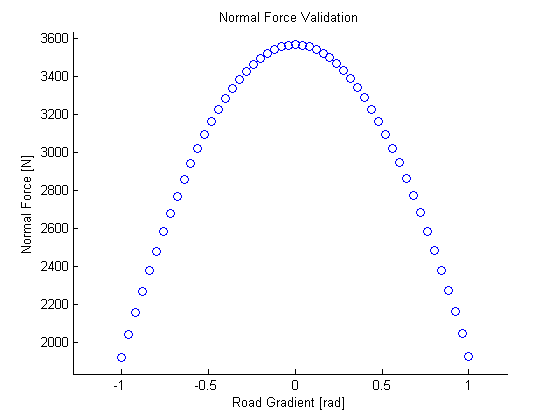
\includegraphics[scale=.75]{chassis_val_normal}
  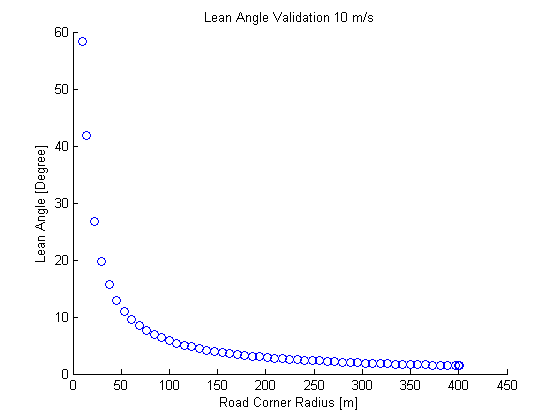
\includegraphics[scale=.75]{chassis_val_leanangle}
  \caption{Chassis Validation}
\end{figure}

Then the Chassis model was validated by simulating a coast down and comparing it against collected data. The data follows the simulation well, but the CdA value needs better calibrated

\begin{figure}[H]
\center
 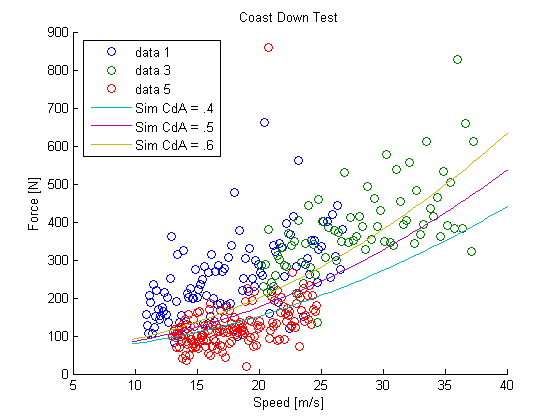
\includegraphics[scale=1]{chassis_val_coastdown}
  \caption{Chassis Validation Coast Down}
\end{figure}



\end{document}